% --------------------------------------------------------------------------
% Mondrian template for LaTeX Beamer presentations
% Author: Janderson Gomes (Caraumã)
% Website: https://carauma.com
% Github: https://github.com/carauma7/latex-presentation-template
% Free and open-source template for LaTeX presentations
% License: Creative Commons Attribution 4.0 International (CC BY 4.0)
% --------------------------------------------------------------------------
\documentclass[aspectratio=169,10pt]{beamer}

\usepackage[utf8]{inputenc}
\usepackage[T1]{fontenc}
\usepackage[english]{babel}
\usepackage{helvet}
\renewcommand{\familydefault}{\sfdefault}
\usepackage{amsmath,amssymb}
\usepackage{booktabs,array,multirow}
\usepackage{tikz,pgfplots}
\pgfplotsset{compat=1.16}
\usetikzlibrary{calc,arrows.meta,positioning}
\usepackage{listings}

% --------------------------------------------------------------------------
% EDITABLE DATA: replace the text inside braces with your presentation data.
% These commands are also used in the footer and title slide.
% --------------------------------------------------------------------------
\newcommand{\authorname}{Your Name}
\newcommand{\coursename}{Course name}
\newcommand{\advisorname}{Advisor or instructor name}
\newcommand{\programname}{Program or course name}
\newcommand{\researchline}{Research line or class}
\newcommand{\institutionname}{Institution name}
\newcommand{\presentationdate}{Month 2026}
\newcommand{\presentationtitle}{Title}
\newcommand{\presentationsubtitle}{A short optional subtitle}
\newcommand{\authorwebsite}{carauma.com}
\newcommand{\shortlicense}{CC BY 4.0}
\newcommand{\longlicense}{Creative Commons Attribution 4.0 International}

% Mondrian color palette
\definecolor{mred}{RGB}{200,52,45}
\definecolor{mblue}{RGB}{36,82,158}
\definecolor{myel}{RGB}{242,201,76}
\definecolor{mgold}{RGB}{206,160,24}
\definecolor{mink}{RGB}{28,28,28}
\definecolor{mpaper}{RGB}{252,251,247}
\definecolor{mgrey}{RGB}{120,120,115}
\colorlet{seccol}{mred}
\colorlet{seccolb}{myel}
\newcommand{\setsec}[2]{\colorlet{seccol}{#1}\colorlet{seccolb}{#2}}

% Theme
\setbeamertemplate{navigation symbols}{}
\setbeamercolor{normal text}{fg=mink,bg=mpaper}
\setbeamercolor{structure}{fg=mink}
\setbeamercolor{block title}{fg=white,bg=mblue}
\setbeamercolor{block body}{fg=mink,bg=mpaper}
\setbeamercolor{block title alerted}{fg=white,bg=mred}
\setbeamercolor{block body alerted}{fg=mink,bg=mpaper}
\setbeamercolor{block title example}{fg=mink,bg=myel}
\setbeamercolor{block body example}{fg=mink,bg=mpaper}
\setbeamerfont{block title}{size=\footnotesize,series=\bfseries}
\setbeamersize{text margin left=1.1cm,text margin right=1.9cm}
\setbeamertemplate{itemize item}{\raisebox{0.15ex}{\textcolor{seccol}{\rule{0.55ex}{0.55ex}}}}
\setbeamertemplate{itemize subitem}{\raisebox{0.15ex}{\textcolor{mink}{\rule{0.4ex}{0.4ex}}}}
\setbeamertemplate{enumerate item}{\insertenumlabel.}
\setbeamercolor{enumerate item}{fg=mink}
\setbeamertemplate{bibliography item}[text]
\setbeamercolor{bibliography item}{fg=mink}
\setbeamerfont{bibliography item}{size=\tiny}
\setbeamerfont{bibliography entry author}{size=\tiny}
\setbeamerfont{bibliography entry title}{size=\tiny}
\setbeamerfont{bibliography entry location}{size=\tiny}
\setbeamerfont{bibliography entry note}{size=\tiny}

\setbeamertemplate{background canvas}{%
 \begin{tikzpicture}[remember picture,overlay]
  \fill[mpaper] (current page.south west) rectangle (current page.north east);
  \fill[mink] ($(current page.north east)+(-1.45,0)$) rectangle
    ($(current page.south east)+(-1.35,0)$);
  \fill[seccol] ($(current page.north east)+(-1.35,0)$) rectangle
    ($(current page.north east)+(0,-1.55)$);
  \fill[mink] ($(current page.north east)+(-1.35,-1.55)$) rectangle
    ($(current page.north east)+(0,-1.65)$);
  \fill[mink] ($(current page.south east)+(-1.35,1.25)$) rectangle
    ($(current page.south east)+(0,1.35)$);
  \fill[seccolb] ($(current page.south east)+(-1.35,0)$) rectangle
    ($(current page.south east)+(0,1.25)$);
 \end{tikzpicture}}

\setbeamertemplate{frametitle}{%
 \vspace{0.6em}%
 \noindent\raisebox{-0.1ex}{\textcolor{seccol}{\rule{0.9ex}{0.9ex}}}\hspace{0.6em}%
 {\Large\bfseries\color{mink}\insertframetitle\par}%
 \vspace{-0.2em}\noindent{\color{mink}\rule{\linewidth}{1.3pt}}\par\vspace{0.2em}}

\setbeamertemplate{footline}{%
 \leavevmode\hbox to \paperwidth{\hspace*{1.1cm}%
 {\fontsize{6}{7}\selectfont\color{mgrey}\authorname \,·\, \presentationtitle}%
 \hfill{\fontsize{7}{8}\selectfont\color{mink}\insertframenumber\,/\,\inserttotalframenumber}
 \hspace*{1.8cm}}%
 \vskip0.3cm}

% Code blocks: use [fragile] on frames containing lstlisting.
\lstdefinelanguage{plain}{}
\lstdefinestyle{code}{
  language=C, basicstyle=\ttfamily\fontsize{7}{8.5}\selectfont\color{mink},
  keywordstyle=\bfseries\color{mblue}, commentstyle=\itshape\color{mgrey},
  numbers=left, numberstyle=\tiny\color{mgrey}, numbersep=5pt,
  frame=l, rulecolor=\color{mink}, framerule=1.2pt, xleftmargin=11pt,
  showstringspaces=false, columns=fullflexible, keepspaces=true,
  literate={á}{{\'a}}1 {à}{{\`a}}1 {ã}{{\~a}}1 {â}{{\^a}}1 {é}{{\'e}}1
    {ê}{{\^e}}1 {í}{{\'i}}1 {ó}{{\'o}}1 {ô}{{\^o}}1 {õ}{{\~o}}1 {ú}{{\'u}}1
    {ç}{{\c c}}1 {Á}{{\'A}}1 {É}{{\'E}}1 {Ç}{{\c C}}1
    {←}{{$\leftarrow$}}1 {↔}{{$\leftrightarrow$}}1 {≤}{{$\leq$}}1
    {≥}{{$\geq$}}1 {−}{{-}}1 {▷}{{$\triangleright$}}1}
\lstdefinestyle{pseudo}{style=code,language=plain,
  basicstyle=\fontsize{7.6}{9.3}\selectfont\color{mink},escapechar=|}
\lstdefinestyle{codesmall}{style=code,
  basicstyle=\ttfamily\fontsize{6.4}{7.8}\selectfont\color{mink}}
\newcommand{\kw}[1]{\textbf{#1}}
\newcommand{\tagbox}[3]{\colorbox{#1}{\textcolor{#2}{\strut\scriptsize\bfseries\ #3\ }}}
\newcommand{\pv}[1]{\colorbox{mred}{\textcolor{white}{\strut\bfseries #1}}}

% Figures: if the file does not exist, a placeholder is drawn.
\newcommand{\figbox}[4]{%
 \IfFileExists{#1}{\includegraphics[width=#2,height=#3,keepaspectratio]{#1}}{%
 \begin{tikzpicture}
  \draw[mink,dashed,line width=0.7pt] (0,0) rectangle (#2,#3);
  \node[text width=\dimexpr#2-0.6cm\relax,align=center,
    font=\scriptsize,text=mgrey] at ({\dimexpr#2/2\relax},{\dimexpr#3/2\relax}) {#4};
 \end{tikzpicture}}}

% Vector diagrams: \qarr{values}{i}{s}{p}, \carr{value/color/text}
\newcommand{\qarr}[4]{%
 \begin{tikzpicture}[baseline=(b.base)]
  \node (b) at (0,0) {\strut};
  \foreach \v [count=\k from 0] in {#1}{%
    \def\cf{mpaper}\def\ct{mink}%
    \ifnum\k<#3 \def\cf{mblue}\def\ct{white}\fi
    \ifnum\k=#2 \def\cf{myel}\def\ct{mink}\fi
    \ifnum\k=#4 \def\cf{mred}\def\ct{white}\fi
    \node[draw=mink,line width=0.8pt,fill=\cf,minimum size=0.7cm,inner sep=0pt,
      text=\ct,font=\bfseries] at (\k*0.86,0) {\v};}%
  \ifnum#2<7 \node[font=\scriptsize\itshape] at (#2*0.86,0.58) {$i$};\fi
  \ifnum#3<7 \node[font=\scriptsize\itshape] at (#3*0.86,-0.58) {$s$};\fi
 \end{tikzpicture}}
\newcommand{\carr}[1]{%
 \begin{tikzpicture}[baseline=(b.base)]
  \node (b) at (0,0) {\strut};
  \foreach \v/\c/\t [count=\k from 0] in {#1}{%
    \node[draw=mink,line width=0.8pt,fill=\c,minimum size=0.7cm,inner sep=0pt,
      text=\t,font=\bfseries] at (\k*0.86,0) {\v};}%
 \end{tikzpicture}}
\newcommand{\tarr}[4]{%
 \begin{tikzpicture}[baseline=(b.base)]
  \node (b) at (0,0) {\strut};
  \foreach \v [count=\k from 0] in {#1}{%
    \def\cf{mpaper}\def\ct{mink}%
    \ifnum\k<#3 \def\cf{myel}\def\ct{mink}\fi
    \ifnum\k<#2 \def\cf{mblue}\def\ct{white}\fi
    \ifnum\k>#4 \def\cf{mred}\def\ct{white}\fi
    \node[draw=mink,line width=0.8pt,fill=\cf,minimum size=0.7cm,inner sep=0pt,
      text=\ct,font=\bfseries] at (\k*0.86,0) {\v};}%
  \node[font=\scriptsize\itshape] at (#3*0.86,0.58) {$i$};
  \node[font=\scriptsize\itshape] at (#2*0.86,-0.58) {$lt$};
  \node[font=\scriptsize\itshape] at (#4*0.86,-0.58) {$gt$};
 \end{tikzpicture}}

% Charts and markers
\pgfplotsset{mond/.style={axis lines=left,axis line style={mink,line width=1pt},
  tick style={mink},tick label style={font=\tiny},label style={font=\scriptsize},
  title style={font=\scriptsize\bfseries},
  legend style={font=\tiny,draw=none,fill=none},
  every axis plot/.append style={line width=1pt}}}
\newcommand{\nb}[3]{\tikz[baseline=-0.6ex]\node[fill=#1,text=#2,minimum size=0.55cm,
  inner sep=0pt,font=\bfseries\small]{#3};}
\newcommand{\ev}[5]{%
 \fill[#3] (#1-0.17,-0.17) rectangle (#1+0.17,0.17);
 \draw[mink,line width=0.6pt] (#1,#2*0.17) -- (#1,#2*0.62);
 \ifnum#2>0 \node[anchor=south,text width=2.4cm,align=center,font=\tiny]
   at (#1,0.65) {\textbf{#4}\\#5};
 \else \node[anchor=north,text width=2.4cm,align=center,font=\tiny]
   at (#1,-0.65) {\textbf{#4}\\#5};\fi}
\newcommand{\chip}[1]{\tikz[baseline=0.05ex]\draw[mink,line width=0.6pt,fill=#1]
  (0,0) rectangle (0.27,0.27);}

% Section opener
\newcommand{\secslide}[6]{%
 \begin{frame}[plain]
  \begin{tikzpicture}[remember picture,overlay]
   \begin{scope}[shift={(current page.south west)}]
    \fill[mpaper] (0,0) rectangle (16,9);
    \fill[#3] (0,6.34) rectangle (3.0,9);
    \fill[#4] (12.74,0) rectangle (16,1.46);
    \fill[#5] (12.74,6.34) rectangle (16,9);
    \fill[mink] (3.0,0) rectangle (3.14,9);
    \fill[mink] (12.6,0) rectangle (12.74,9);
    \fill[mink] (0,6.2) rectangle (16,6.34);
    \fill[mink] (3.14,1.46) rectangle (16,1.6);
    \node[text=#6,font=\fontsize{44}{44}\bfseries] at (1.5,7.7) {#1};
    \node[anchor=west,text width=8.6cm,align=left,font=\fontsize{24}{28}\bfseries,
      text=mink] at (3.6,3.6) {#2};
   \end{scope}
  \end{tikzpicture}
 \end{frame}}

\title{\presentationtitle}
\begin{document}

% Title slide
\begin{frame}[plain]
 \begin{tikzpicture}[remember picture,overlay]
  \begin{scope}[shift={(current page.south west)}]
   \fill[mpaper] (0,0) rectangle (16,9);
   \fill[mred] (0,6.64) rectangle (3.0,9);
   \fill[myel] (13.14,6.64) rectangle (16,9);
   \fill[mblue] (13.14,0) rectangle (16,1.86);
   \fill[mink] (3.0,0) rectangle (3.14,9);
   \fill[mink] (13.0,0) rectangle (13.14,9);
   \fill[mink] (0,6.5) rectangle (16,6.64);
   \fill[mink] (3.14,1.72) rectangle (16,1.86);
   \fill[mink] (0,4.3) rectangle (3.0,4.44);
   \node[anchor=west,font=\scriptsize\bfseries,text=mgrey,text width=9.5cm]
     at (3.5,7.9) {\MakeUppercase{\institutionname}\\[2pt]
     \MakeUppercase{\programname}\\\MakeUppercase{\researchline}};
   \node[anchor=west,font=\fontsize{40}{44}\bfseries,text=mink,text width=9.2cm]
     at (3.5,5.25) {\presentationtitle};
   \node[anchor=west,font=\large,text=mgrey,text width=9.2cm]
     at (3.5,3.65) {\presentationsubtitle};
   \node[anchor=west,font=\small,text=mink,text width=9.2cm] at (3.5,2.45)
     {\textbf{\authorname}};
   \node[anchor=west,font=\small,text=mink,text width=9.2cm] at (3.5,0.75)
     {\textbf{\coursename} \,|\, \advisorname \,|\,  \presentationdate};
   \node[anchor=west,font=\fontsize{5.5}{6.5}\selectfont,text=mgrey,text width=9.2cm]
     at (3.5,0.28) {\copyright\ 2026 Janderson Gomes (Caraumã) \,·\,
     \href{https://creativecommons.org/licenses/by/4.0/}{\longlicense} \,·\, \href{https://carauma.com}{\authorwebsite}};
  \end{scope}
 \end{tikzpicture}
\end{frame}

% Editable agenda
\begin{frame}{Contents}
 \begin{columns}[T]
  \column{0.49\textwidth}
   \vspace{0.4em}
   \nb{mred}{white}{1}\ \ Context and motivation\\[1.1ex]
   \nb{mblue}{white}{2}\ \ Main concept\\[1.1ex]
   \nb{myel}{mink}{3}\ \ Step-by-step example\\[1.1ex]
   \nb{mred}{white}{4}\ \ Implementation
  \column{0.49\textwidth}
   \vspace{0.4em}
   \nb{mblue}{white}{5}\ \ Results\\[1.1ex]
   \nb{myel}{mink}{6}\ \ Comparisons\\[1.1ex]
   \nb{mred}{white}{7}\ \ Applications\\[1.1ex]
   \nb{mblue}{white}{8}\ \ Conclusion
 \end{columns}
\end{frame}

\setsec{mred}{myel}
\secslide{1}{Context\\and motivation}{mred}{mblue}{myel}{white}

\begin{frame}{Slide title}
 \begin{columns}[T]
  \column{0.56\textwidth}
   \small This is sample text. Replace this paragraph with a concise
   explanation of the problem, context, or question guiding your presentation.
   \vspace{0.4em}
   \begin{itemize}
    \item \textbf{Main point:} describe the first idea.
    \item \textbf{Evidence:} add a data point or reference.
    \item \textbf{Goal:} state the expected outcome.
   \end{itemize}
  \column{0.3035\textwidth}
   \begin{exampleblock}{Highlight}
    \footnotesize Use this block for a definition, hypothesis, or message
    that you want to emphasize visually.
   \end{exampleblock}
 \end{columns}
\end{frame}

\begin{frame}{Timeline or sequence}
 \centering
 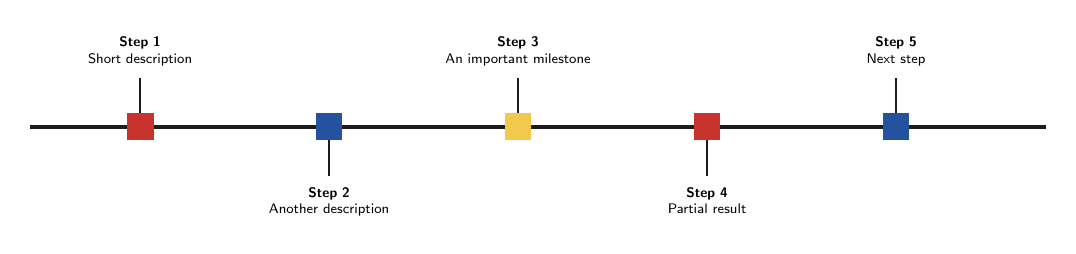
\begin{tikzpicture}[x=1cm,y=1cm]
  \draw[mink,line width=1.6pt] (0,0) -- (12.9,0);
  \ev{1.4}{1}{mred}{Step 1}{Short description}
  \ev{3.8}{-1}{mblue}{Step 2}{Another description}
  \ev{6.2}{1}{myel}{Step 3}{An important milestone}
  \ev{8.6}{-1}{mred}{Step 4}{Partial result}
  \ev{11.0}{1}{mblue}{Step 5}{Next step}
 \end{tikzpicture}
\end{frame}

\setsec{mblue}{mred}
\secslide{2}{Main concept}{mblue}{myel}{mred}{white}

\begin{frame}{TikZ diagram}
 \begin{columns}[T]
  \column{0.44\textwidth}
   \begin{enumerate}
    \item \textbf{Input}: data or assumptions.
    \item \textbf{Processing}: main transformation.
    \item \textbf{Output}: result or decision.
   \end{enumerate}
  \column{0.52\textwidth}
   \centering
   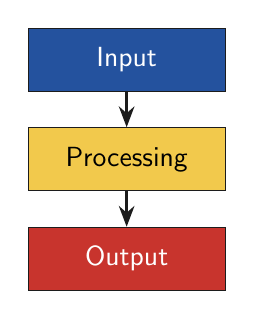
\begin{tikzpicture}[node distance=0.45cm]
    \node[draw=mink,fill=mblue,text=white,minimum width=2.5cm,
      minimum height=0.8cm] (a) {Input};
    \node[draw=mink,fill=myel,minimum width=2.5cm,
      minimum height=0.8cm,below=of a] (b) {Processing};
    \node[draw=mink,fill=mred,text=white,minimum width=2.5cm,
      minimum height=0.8cm,below=of b] (c) {Output};
    \draw[-{Stealth},mink,line width=1pt] (a) -- (b);
    \draw[-{Stealth},mink,line width=1pt] (b) -- (c);
   \end{tikzpicture}
 \end{columns}
\end{frame}

\begin{frame}[fragile]{Code example}
 \begin{columns}[T]
  \column{0.46\textwidth}
   \tagbox{mblue}{white}{Pseudocode}\vspace{0.3em}
\begin{lstlisting}[style=pseudo]
PROCESS(data)
1  | \kw{for each} | item | \kw{in} | data | \kw{do} |
2      transform(item)
3  | \kw{return} | result
\end{lstlisting}
  \column{0.48\textwidth}
   \tagbox{mred}{white}{C language}\vspace{0.3em}
\begin{lstlisting}[style=code]
int process(int data[], int n) {
    int result = 0;
    for (int i = 0; i < n; i++)
        result += data[i];
    return result;
}
\end{lstlisting}
 \end{columns}
\end{frame}

\setsec{myel}{mblue}
\secslide{3}{Step-by-step\\example}{myel}{mred}{mblue}{mink}

\begin{frame}{Vector visualization}
 \centering
 \vspace{0.8em}
 \qarr{8,3,6,1,5,2}{2}{2}{5}
 \par\vspace{1em}
 \carr{A/mred/white,B/mblue/white,C/myel/mink,D/mpaper/mink}
 \par\vspace{1em}
 \tarr{4,2,4,1,4,3}{1}{3}{4}
 \par\vspace{1em}
 {\scriptsize Use \texttt{\textbackslash qarr}, \texttt{\textbackslash carr}, and
 \texttt{\textbackslash tarr} to create editable vector diagrams.}
\end{frame}

\begin{frame}{Table and message blocks}
 \begin{columns}[T]
  \column{0.48\textwidth}
   \centering\footnotesize
   \renewcommand{\arraystretch}{1.25}
   \begin{tabular}{@{}lcc@{}}
    \toprule
    \textbf{Item} & \textbf{Before} & \textbf{After}\\
    \midrule
    A & 12 & 18\\
    B & 8 & 11\\
    C & 15 & 13\\
    \bottomrule
   \end{tabular}
  \column{0.42\textwidth}
   \begin{block}{Partial conclusion}
    \footnotesize The blue block can present an intermediate summary.
   \end{block}
   \begin{alertblock}{Attention}
    \footnotesize The red block draws attention to a limitation.
   \end{alertblock}
 \end{columns}
\end{frame}

\setsec{mred}{mblue}
\secslide{4}{Results\\and comparison}{mred}{mblue}{myel}{white}

\begin{frame}{Editable PGFPlots chart}
 \centering
 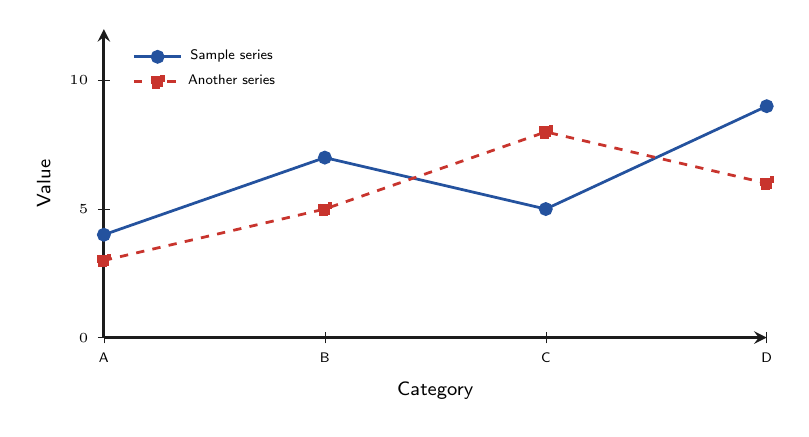
\begin{tikzpicture}
  \begin{axis}[mond,width=10cm,height=5.5cm,xlabel={Category},
    ylabel={Value},ymin=0,ymax=12,xtick={1,2,3,4},
    xticklabels={A,B,C,D},legend pos=north west]
   \addplot[mblue,mark=*] coordinates {(1,4)(2,7)(3,5)(4,9)};
   \addlegendentry{Sample series}
   \addplot[mred,dashed,mark=square*] coordinates {(1,3)(2,5)(3,8)(4,6)};
   \addlegendentry{Another series}
  \end{axis}
 \end{tikzpicture}
\end{frame}

\begin{frame}{Conclusions and next steps}
 \begin{columns}[T]
  \column{0.42\textwidth}
   \begin{block}{What we learned}
    \footnotesize
    \begin{itemize}
     \item Summarize the main discovery.
     \item Relate the result to the goal.
     \item Record a relevant limitation.
    \end{itemize}
   \end{block}
  \column{0.42\textwidth}
   \begin{exampleblock}{Next steps}
    \footnotesize List actions, open questions, or extensions of the work here.
   \end{exampleblock}
 \end{columns}
\end{frame}

% Closing slide
\begin{frame}[plain]
 \begin{tikzpicture}[remember picture,overlay]
  \begin{scope}[shift={(current page.south west)}]
   \fill[mpaper] (0,0) rectangle (16,9);
   \fill[mblue] (0,0) rectangle (3.0,4.2);
   \fill[mred] (13.14,6.64) rectangle (16,9);
   \fill[myel] (13.14,0) rectangle (16,1.86);
   \fill[mink] (3.0,0) rectangle (3.14,9);
   \fill[mink] (13.0,0) rectangle (13.14,9);
   \fill[mink] (0,4.2) rectangle (16,4.34);
   \fill[mink] (3.14,1.72) rectangle (16,1.86);
   \fill[mink] (3.14,6.5) rectangle (16,6.64);
   \node[anchor=west,font=\fontsize{40}{44}\bfseries] at (3.6,5.5) {Thank you!};
   \node[anchor=west,font=\large,text width=8.8cm] at (3.6,3.2)
     {Questions and discussion};
   \node[anchor=west,font=\small,text=mgrey,text width=8.8cm] at (3.6,2.55)
     {\copyright\ 2026 Janderson Gomes (Caraumã) \,·\,
     \href{https://creativecommons.org/licenses/by/4.0/}{\shortlicense}
     \,·\, \href{https://carauma.com}{\authorwebsite}};
  \end{scope}
 \end{tikzpicture}
\end{frame}

\end{document}
